\documentclass{exam}
\usepackage[utf8]{inputenc}
\usepackage{lmodern}
\usepackage{microtype}

% \usepackage[parfill]{parskip}
\usepackage[dvipsnames]{xcolor}
\usepackage{amsmath}
\usepackage{amsfonts}
\usepackage{amsthm}
\usepackage{siunitx}
\DeclareSIUnit\year{yr}
\DeclareSIUnit\foot{ft}
\DeclareSIUnit\litre{\liter}

\usepackage{skull}

\usepackage{pgfplots}
\usepgfplotslibrary{polar}
\pgfplotsset{compat=1.11}
\usepgfplotslibrary{statistics}
\usepackage{graphicx}
\usepackage{sidecap}
\sidecaptionvpos{figure}{c}
\usepackage{float}
\usepackage{gensymb}
\usepackage{tkz-euclide}
\usetkzobj{all}
\usepackage{commath}
\usepackage{hyperref}
\usepackage{enumitem}
\usepackage{wasysym}
\usepackage{multicol}
\usepackage{mathtools}
\usepackage{tcolorbox}
\usepackage{tabularx}
\usepackage[version=4]{mhchem}
\usepackage{changepage}
\usepackage{listings}
\lstset{basicstyle=\ttfamily\linespread{0.8}\small}

\renewcommand*{\thefootnote}{\fnsymbol{footnote}}

\newtheorem*{thm}{Theorem}
\newtheorem*{iden}{Identity}
\newtheorem*{lemma}{Lemma}
\newtheorem{obs}{Observation}
\theoremstyle{definition}
\newtheorem*{defn}{Definition}
\newtheorem*{ex}{Example}
\newtheorem{con}{Construction}
\newtheorem*{alg}{Algorithm}

\newtheoremstyle{break}
  {\topsep}{\topsep}%
  {\itshape}{}%
  {\bfseries}{}%
  {\newline}{}%
\theoremstyle{break}
\newtheorem*{bthm}{Theorem}

% russian integral
\usepackage{scalerel}
\DeclareMathOperator*{\rint}{\scalerel*{\rotatebox{17}{$\!\int\!$}}{\int}}

% \DeclareMathOperator*{\rint}{\int}

\pgfplotsset{vasymptote/.style={
    before end axis/.append code={
        \draw[densely dashed] ({rel axis cs:0,0} -| {axis cs:#1,0})
        -- ({rel axis cs:0,1} -| {axis cs:#1,0});
    }
}}

% \pointsinrightmargin
\boxedpoints
\pointname{}

\newcommand{\questioA}{\question[\texttt{\textbf{\color{Cerulean} A}}]}
\newcommand{\questioM}{\question[\texttt{\textbf{\color{PineGreen} M}}]}
\newcommand{\questioE}{\question[\texttt{\textbf{\color{WildStrawberry} E}}]}
\newcommand{\questioS}{\question[\texttt{\textbf{\color{Goldenrod} S}}]}
\newcommand{\questioO}{\question[\texttt{\textbf{\color{BurntOrange} O}}]}

\newcommand{\parA}{\part[\texttt{\textbf{\color{Cerulean} A}}]}
\newcommand{\parM}{\part[\texttt{\textbf{\color{PineGreen} M}}]}
\newcommand{\parE}{\part[\texttt{\textbf{\color{WildStrawberry} E}}]}
\newcommand{\parS}{\part[\texttt{\textbf{\color{Goldenrod} S}}]}
\newcommand{\parO}{\part[\texttt{\textbf{\color{BurntOrange} O}}]}

\newcommand{\subparA}{\subpart[\texttt{\textbf{\color{Cerulean} A}}]}
\newcommand{\subparM}{\subpart[\texttt{\textbf{\color{PineGreen} M}}]}
\newcommand{\subparE}{\subpart[\texttt{\textbf{\color{WildStrawberry} E}}]}
\newcommand{\subparS}{\subpart[\texttt{\textbf{\color{Goldenrod} S}}]}
\newcommand{\subparO}{\subpart[\texttt{\textbf{\color{BurntOrange} O}}]}

\newcommand{\mainHeader}[2]{\section*{NCEA Level 2 Mathematics\\#1. #2}}
\newcommand{\mainHeaderHw}[2]{\section*{NCEA Level 2 Mathematics (Homework)\\#1. #2}}
\newcommand{\seealso}[1]{\begin{center}\emph{See also #1.}\end{center}}
\newcommand{\drills}[1]{\begin{center}\emph{Drill problems: #1.}\end{center}}
\newcommand{\basedon}[1]{\begin{center}\emph{Notes largely based on #1.}\end{center}}


\begin{document}

\mainHeader{7}{Linear Inequalities}
An equation is a statement which says that two quantities are identical. If we don't want to be so precise, we can talk about
inequalities: statements which tell us about the \emph{relative size} of two quantities. More precisely, if $ a $ and $ b $
are two quantities then:
\begin{center}
  \begin{tabular}{cl}
    $ a = b $ & $ a $ is identical to $ b $\\
    $ a \neq b $ & $ a $ is not identical to $ b $\\
    $ a \leq b $ & either $ a $ is identical to $ b $, or $ a $ is smaller than $ b $\\
    $ a < b $ & $ a $ is not identical to $ b $ and $ a $ is smaller than $ b $
  \end{tabular}
\end{center}

This allows us to impose an \emph{ordering} structure onto the integers, as well as the algebraic structure that they already
had. We will look at the interplay between the two in the exercises.

\subsection*{Questions}
\begin{questions}
  \question Justify the following statements with mathematical reasoning (where $ a$, $ b$, and $c$ are quantities):
    \begin{parts}
      \part Precisely one of $ a < b $, $ a = b $, or $ a > b $ is true.
      \part If $ a \leq b $ and $ b \leq c $ then $ a \leq c $.
      \part If $ a \leq b $ and $ b \leq a $ then $ a = b $.
    \end{parts}
  \question Using number lines, explain why
    \begin{parts}
      \part $ (-3) + (-4) = -7 $;
      \part $ (-2) + 4 = 2 $;
      \part $ (-10) + 4 = -6 $.
    \end{parts}
  \question Consider the following multiplication table.
            \begin{center}
              \def\arraystretch{1.5}
              \begin{tabular}{|ccc|c|}\hline
                $ a $ && $ b $ & $ ab $\\\hline
                $ 2 $ & $ \times $ & $ 5 $ & $ 10 $\\\hline
                $ 2 $ & $ \times $ & $ 4 $ & $ 8 $\\\hline
                $ 2 $ & $ \times $ & $ 3 $ & $ 6 $\\\hline
                $ 2 $ & $ \times $ & $ 2 $ & $ 4 $\\\hline
                $ 2 $ & $ \times $ & $ 1 $ & $ 2 $\\\hline
                $ 2 $ & $ \times $ & $ 0 $ & $ 0 $\\\hline\hline
                $ 2 $ & $ \times $ & $ -1 $ &\\\hline
                $ 2 $ & $ \times $ & $ -2 $ &\\\hline\hline
                $ 2 $ & $ \times $ & $ -10 $ &\\\hline
              \end{tabular}
            \end{center}
    \begin{parts}
      \part What is the pattern in the final column?
      \part Fill in the final three lines of the table by continuing the pattern.
      \part Based on this table, is it more reasonable for the product of a \textbf{negative by a positive} to be positive or negative?
      \part Using this definition, fill in the first five lines of the next table:
            \begin{center}
              \def\arraystretch{1.5}
              \begin{tabular}{|ccc|c|}\hline
                $ a $ && $ b $ & $ ab $\\\hline
                $ -3 $ & $ \times $ & $ 4 $ & \\\hline
                $ -3 $ & $ \times $ & $ 3 $ & \\\hline
                $ -3 $ & $ \times $ & $ 2 $ & \\\hline
                $ -3 $ & $ \times $ & $ 1 $ & \\\hline
                $ -3 $ & $ \times $ & $ 0 $ & \\\hline\hline
                $ -3 $ & $ \times $ & $ -1 $ &\\\hline
                $ -3 $ & $ \times $ & $ -2 $ &\\\hline\hline
                $ -3 $ & $ \times $ & $ -10 $ &\\\hline
              \end{tabular}
            \end{center}
      \part Again using the pattern we see as we move down the final column, fill in the last three rows.
      \part Based on this table, is it more reasonable for the product of a \textbf{negative by a negative} to be positive or negative?
    \end{parts}
  \question Justify the following statements with mathematical reasoning (where $ a$, $ b$, $c$, and $ d $ are quantities) --- you may want to draw
            number lines, it makes things easier to visualise:
    \begin{parts}
      \part If $ a \leq b $ and $ c $ is \emph{positive} then $ ac \leq bc $.
      \part If $ a \leq b $ and $ c $ is \emph{negative} then $ ac \geq bc $.
      \part If $ a \leq b $ and $ c $ is any quantity then $ a + c \leq b + c $.
      \part If $ a \leq b $ and $ c \leq d $ then $ a + c \leq b + d $.
      \part If $ a \leq b $ and $ c \leq d $ then we cannot make any statement about the relative values of $ a + d $ and $ b + c $. [Hint: consider $ 1 \leq 2 $
            and $ 1 \leq 1 $ as $ a \leq b $ and $ c \leq d $ respectively, then swap them around.]
    \end{parts}
  \question We will now look at inequalities which involve variables.
    \begin{parts}
      \part For each of the following inequations, graph all the possible values of $ x $ and $ y $ that satisfy it.
        \begin{subparts}
          \subpart $ 4 + x < 3 $
          \subpart $ 3x + 2 \geq 2 $
          \subpart $ x \geq y $
          \subpart $ x \leq y $
          \subpart $ 3x + 9y \leq 1 $
          \subpart $ 2x + y \geq 0 $
        \end{subparts}
      \part Graph all possible values of $ x $ and $ y $ satisfying each of the following \emph{sets} of inequalities. (The resulting region of the plane is
            called the \emph{feasible region} of the system.)
        \begin{subparts}
          \subpart $ x < y $, $ x > y $, and $ x < 2y $
          \subpart $ x \leq 2 $, $ x \geq -1 $, $ y \leq x $, $ y \geq x - 3 $
        \end{subparts}
    \end{parts}
  \clearpage
  \question Consider the following graphed system of inequalities.
            \begin{center}
              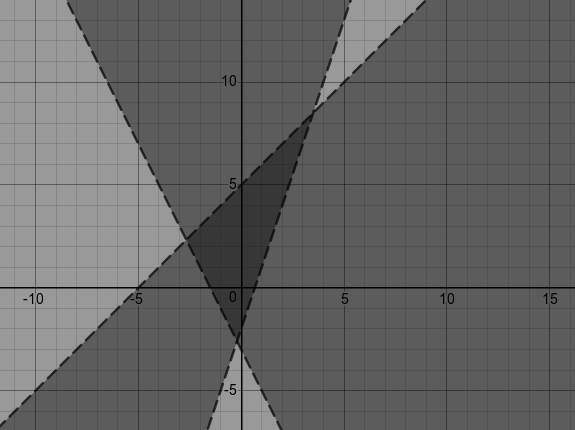
\includegraphics[width=0.5\textwidth]{lineqs}
            \end{center}
    \begin{parts}
      \part Explicitly write down the three inequalities that have been graphed.
      \part What are the coordinates of the three intersection points?
    \end{parts}
  \question
    \begin{parts}
      \part Show that no point simultaneously satisfies both of $ y \geq 2x + 1 $ and $ y \leq 2x - 3 $.
      \part Show that if $ y \leq Ax + B $ is any linear inequality in $ x $ and $ y $, then the feasible region
            of this inequality overlaps with at least one of the inequalities in (a).
    \end{parts}
  \question The \textbf{arithmetic mean} of two numbers $ a $ and $ b $ is $ \frac{a + b}{2} $; the \textbf{geometric mean}
            of $ a $ and $ b $ is $ \sqrt{ab} $.
    \begin{parts}
      \part Calculate the arithmetic and geometric means for several pairs of numbers. Make a conjecture about
            the relative order of the two means (is one always bigger than the other)?
      \part Show that
            \begin{displaymath}
              \left(\frac{a + b}{2}\right)^2 - ab = \left(\frac{a - b}{2}\right)^2.
            \end{displaymath}
      \part Suppose that $ a $ and $ b $ are positive numbers. Using part (b), or otherwise, show that the
            geometric mean of $ a $ and $ b $ is always less than or equal to their arithmetic mean. When
            are the two equal?
      \part Investigate the cases where $ a $ and $ b $ are both negative, or one is negative and one is positive. (Hint: one
            of these cases makes no sense.)
    \end{parts}
\end{questions}

\end{document}
